\documentclass[11pt,a4paper]{article}

\usepackage[T1]{fontenc}
\usepackage[utf8]{inputenc}
\usepackage{lmodern}
\usepackage{microtype}
\usepackage[a4paper,margin=2.4cm]{geometry}
\usepackage{amsmath,amssymb,bm}
\usepackage{graphicx}
\usepackage{booktabs}
\usepackage{array}
\usepackage{float}
\usepackage{caption}
\usepackage{subcaption}
\usepackage{xcolor}
\usepackage{enumitem}
\usepackage{fancyhdr}
\usepackage{hyperref}
\usepackage{listings}

\newcommand{\studentname}{Grigory Guliy} % replace with your name

\hypersetup{
  colorlinks=true,
  linkcolor=black,
  citecolor=black,
  urlcolor=blue,
  pdftitle={A shock-capturing shallow-water solver in OpenFOAM},
  pdfauthor={\studentname}
}
\captionsetup{font=small, labelfont=bf, labelsep=period, skip=6pt}
\setlength{\parskip}{4pt}
\setlength{\parindent}{0pt}

\pagestyle{fancy}
\fancyhf{}
\fancyhead[L]{\small Skoltech. F2026. Modeling with Open Source Software. Project report.}
\fancyhead[R]{\small By \studentname}
\fancyfoot[C]{\small\thepage}
\renewcommand{\headrulewidth}{0.4pt}

\newcommand{\Froude}{\mathrm{Fr}}
\newcommand{\Rey}{\mathrm{Re}}
\newcommand{\We}{\mathrm{We}}
\newcommand{\Bo}{\mathrm{Bo}}
\newcommand{\bU}{\mathbf{U}}
\newcommand{\bu}{\mathbf{u}}
\newcommand{\bn}{\mathbf{n}}
\newcommand{\bx}{\mathbf{x}}
\newcommand{\bF}{\mathbf{F}}
\newcommand{\bQ}{\mathbf{Q}}
\newcommand{\bS}{\mathbf{S}}
\newcommand{\bI}{\mathbf{I}}
\newcommand{\dt}{\Delta t}
\newcommand{\dx}{\Delta x}
\newcommand{\dy}{\Delta y}
\newcommand{\dr}{\Delta r}
\newcommand{\Order}{\mathcal{O}}

\lstset{
  basicstyle=\ttfamily\scriptsize,
  numbers=left,
  numberstyle=\tiny,
  stepnumber=1,
  frame=single,
  breaklines=true,
  columns=fullflexible,
  keepspaces=true,
  showstringspaces=false,
  captionpos=b
}

\begin{document}

%-----------------------------------------------------------------------
\begin{titlepage}
\centering
\vspace*{2.2cm}
{\LARGE\bfseries A shock-capturing shallow-water solver in OpenFOAM\par}
\vspace{0.5cm}
{\Large Verification and the two-dimensional radial dam break\par}
\vspace{2.2cm}
{\large A term project in the course:\\[2pt]
Modeling with Open Source Software\par}
\vspace{1.2cm}
{\large Progress report\par}
\vspace{2.2cm}
{\large by \studentname\\[2pt]
Skoltech, Fall 2026\par}
\vfill
{\large \today\par}
\end{titlepage}

\pagenumbering{arabic}
\thispagestyle{fancy}

\noindent\textbf{Abstract.}
This progress report describes a compact, explicit finite-volume solver for the
two-dimensional shallow-water equations, implemented as an OpenFOAM
application and verified on the classical dam-break problem.  The numerical
scheme combines an HLL or HLLC Riemann flux, MUSCL reconstruction with a
Barth--Jespersen limiter, forward-Euler time integration, a CFL condition, and
a positivity/dry-bed treatment.  A one-dimensional $r$-weighted axisymmetric
mode is included for the radial dam break.  The wet dam break reproduces the
Stoker plateau and shock to within $0.01\%$ in depth and velocity, the
nearly-dry case to within $0.1\%$, and the dry case remains positive and
mass-conservative, although its front is smeared by numerical diffusion.  A
grid-convergence study gives an observed $L_1$ order of about $0.9$, consistent
with first-order convergence of a shock-dominated solution.  The 1D
axisymmetric radial solution is stable and mass-conservative.  Its 2D
Cartesian counterpart on a $400\times400$ mesh is exactly axisymmetric,
conserves mass to $1.2\times10^{-10}$ relative error, and reproduces the 1D
radial front at $r=5.625$ m versus $5.6275$ m.  The main limitations are the
small stable CFL number, the diffusive dry front, a residual oscillation in the
radial velocity on the outer plateau, and the coarse 2D mesh.  The final report
will add the Clawpack $2:1$ radial benchmark and a systematic 2D mesh-refinement
study.

\section{Introduction}

\subsection{Problem and motivation}
A dam break is the canonical hyperbolic test for shallow-water models.  A
column of water of depth $h_L$ is released into an ambient layer of depth
$h_R$; the solution immediately develops a rarefaction wave, a constant
plateau, and a bore (shock).  The same mathematical structure appears in
flood-wave propagation, dam-safety analysis, tsunami run-up, and coastal
engineering.  The depth-averaged shallow-water equations (SWE) are the standard
model for these large-scale flows: they are hyperbolic, nonlinear, and admit
discontinuous solutions even from smooth initial data.

The project has two goals.  The first is to build a small, understandable,
shock-capturing SWE solver inside OpenFOAM, using the same fields
(\texttt{h}, \texttt{hU}), meshes, and boundary-condition machinery as the rest
of the environment, but replacing the pressure-based PISO/PIMPLE algorithm by
an explicit Godunov-type finite-volume method.  The second is to verify this
solver quantitatively against the classical Ritter and Stoker solutions and to
use it for a 2D radial dam break, which is a preliminary step toward a
two-dimensional shock-capturing shallow-water capability.

The native OpenFOAM solver \texttt{shallowWaterFoam} is pressure-based: it
solves a Poisson equation for the free-surface elevation and is not a Riemann
solver.  In the first stage of the project it was run on the same one-dimensional
pipe.  The wet $10:1$ case matched Stoker reasonably well, but the dry case
failed at initialisation because $U=hU/h$ gives $0/0$ when $h=0$, and the
nearly-dry $1$~mm case failed at $t\approx16.7$~s when $h$ became negative and
the solver evaluated $\sqrt{h}$.  These failures are the direct motivation for
the explicit, positivity-preserving solver described here.

\subsection{State of the art}
Godunov-type finite-volume methods are the standard tool for hyperbolic
conservation laws.  The HLL approximate Riemann solver of Harten, Lax and
van Leer \cite{harten1983} is robust and positivity-preserving for the SWE,
while the HLLC variant of Toro, Spruce and Speares \cite{toro1994} restores the
contact/shear wave and is sharper in two dimensions.  Second-order accuracy in
smooth regions is obtained with MUSCL reconstruction \cite{vanleer1979} and a
TVD limiter; the Barth--Jespersen limiter \cite{barth1989} is a convenient
multidimensional choice.  Dry and nearly-dry states require additional care:
hydrostatic reconstruction and well-balanced schemes \cite{audusse2004,
kurganov2007,bollermann2013} preserve the lake-at-rest state and avoid
negative depths.  The Clawpack/GeoClaw ecosystem \cite{mandli2016} and the
SWASHES benchmark library \cite{delestre2013} provide independent numerical
and analytical references.  OpenFOAM itself \cite{weller1998,openfoam2406}
supplies the mesh, fields, and I/O infrastructure.

\subsection{Questions and outline}
The report addresses four questions:
(i) can a compact OpenFOAM implementation of HLL/HLLC plus MUSCL reproduce the
Stoker and Ritter solutions quantitatively?
(ii) does the positivity/dry-bed treatment keep the depth non-negative and the
mass conserved on dry and nearly-dry beds?
(iii) does the $r$-weighted axisymmetric form reproduce the 1D radial dam break?
(iv) does the 2D Cartesian solver produce an axisymmetric radial dam break that
agrees with the 1D radial reference?

Section~\ref{sec:math} presents the governing equations, assumptions, initial
and boundary conditions, and the exact/reference solutions.  Section~\ref{sec:dim}
performs the dimensional analysis.  Section~\ref{sec:num} describes the
finite-volume discretisation, Riemann solvers, reconstruction, time stepping,
positivity treatment, radial source, and boundary conditions.
Section~\ref{sec:setup} specifies the computational cases and numerical
settings.  Section~\ref{sec:results} presents the preliminary verification,
grid-convergence, 1D radial, and 2D radial results, and discusses their
limitations.  Section~\ref{sec:conclusions} concludes and outlines the final
report.

%-----------------------------------------------------------------------
\section{Mathematical formulation}
\label{sec:math}

\subsection{Model assumptions}
The SWE are obtained from the incompressible Euler equations with a free
surface under the following assumptions:
\begin{enumerate}[leftmargin=1.4em,itemsep=1pt,topsep=2pt]
\item the flow is incompressible and of constant density $\rho$;
\item the vertical acceleration is negligible and the pressure is hydrostatic,
      $p=\rho g(\eta-z)$, where $\eta$ is the free-surface elevation;
\item the horizontal velocity is approximately uniform over the depth, so the
      equations are depth-averaged;
\item the bed is flat, $b(x,y)=0$, and friction, Coriolis, and viscous effects
      are neglected;
\item the horizontal length scale $L$ is much larger than the depth $H$, so the
      long-wave (shallow-water) approximation holds.
\end{enumerate}
The last assumption is the one that restricts the model to long waves; it is
reasonable for a dam break at the metre scale, but it excludes dispersive
(non-hydrostatic) effects, which are outside the scope of this project.

\subsection{Governing equations}
Let $h(\bx,t)$ be the water depth and $\bu(\bx,t)=(u,v)$ the depth-averaged
horizontal velocity.  The two-dimensional SWE in conservative form are
\begin{align}
  \partial_t h + \nabla\cdot(h\bu) &= 0, \label{eq:mass}\\
  \partial_t(h\bu) + \nabla\cdot\left(h\bu\otimes\bu
      + \frac{g h^2}{2}\bI\right) &= -g h\nabla b, \label{eq:mom}
\end{align}
with $g=9.81$~m~s$^{-2}$ and $b=0$ in this work.  The flux vector in a
direction $\bn$ is
\begin{equation}
  \bF_n(h,\bu) =
  \begin{pmatrix}
    h u_n\\[2pt]
    h u_n \bu + \dfrac{g h^2}{2}\bn
  \end{pmatrix},
  \qquad u_n=\bu\cdot\bn .
  \label{eq:flux}
\end{equation}
The source term on the right-hand side of \eqref{eq:mom} vanishes for a flat
bed.  In primitive variables the same equations read
\begin{equation}
  \partial_t h + \bu\cdot\nabla h + h\nabla\cdot\bu = 0,\qquad
  \partial_t\bu + (\bu\cdot\nabla)\bu + g\nabla h = 0 .
  \label{eq:primitive}
\end{equation}
The Jacobian of $\bF_n$ has the eigenvalues
\begin{equation}
  \lambda_1=u_n-c,\qquad \lambda_2=u_n,\qquad \lambda_3=u_n+c,
  \qquad c=\sqrt{g h},
  \label{eq:eigen}
\end{equation}
so the system is hyperbolic for $h>0$.  In one dimension the Riemann
invariants are $u+2c$ and $u-2c$ along the characteristics
$\mathrm{d}x/\mathrm{d}t=u\pm c$.

\subsection{One-dimensional and axisymmetric forms}
For the pipe cases the solution is uniform in $y$, and the one-dimensional SWE
are
\begin{align}
  \partial_t h + \partial_x(hu) &= 0, \label{eq:1dmass}\\
  \partial_t(hu) + \partial_x\left(hu^2+\frac{g h^2}{2}\right) &= 0 .
  \label{eq:1dmom}
\end{align}
For the axisymmetric radial dam break, with $r$ the radial coordinate and
$u=u_r$, the equations are
\begin{align}
  \partial_t h + \frac{1}{r}\partial_r(r h u) &= 0, \label{eq:radmass}\\
  \partial_t(hu) + \frac{1}{r}\partial_r(r h u^2) + g h\,\partial_r h &= 0 .
  \label{eq:radmom}
\end{align}
The $1/r$ singularity at the axis is removed by the $r$-weighted conservative
form
\begin{align}
  \partial_t(r h) + \partial_r(r h u) &= 0, \label{eq:rwmass}\\
  \partial_t(r h u) + \partial_r\left(r h u^2+\frac{g}{2}r h^2\right)
  &= \frac{g}{2}h^2 . \label{eq:rwmom}
\end{align}
The geometric source in \eqref{eq:rwmom} is the only place where the radial
geometry enters; the axis condition is $u(0,t)=0$, and the axis face has
$r_f=0$, so its mass and momentum fluxes vanish.

\subsection{Initial and boundary conditions}
\paragraph{One-dimensional pipe.}
The initial state is a dam at $x=0$:
\begin{equation}
  h(x,0)=
  \begin{cases}
    h_L,& x<0,\\
    h_R,& x>0,
  \end{cases}
  \qquad u(x,0)=0 .
  \label{eq:ic1d}
\end{equation}
The wet case uses $(h_L,h_R)=(1.0,0.1)$~m, the dry case $h_R=0$, and the
nearly-dry case $h_R=10^{-3}$~m.  The ends $x=\pm L$ are transmissive
(zero-gradient) in the computations; they are far enough from the dam that the
waves do not reach them during the run, except for the long nearly-dry domain.

\paragraph{Radial 1D.}
The initial state is a circular column of radius $R_0$:
\begin{equation}
  h(r,0)=
  \begin{cases}
    h_L,& r<R_0,\\
    h_R,& r>R_0,
  \end{cases}
  \qquad u(r,0)=0,
  \label{eq:icrad}
\end{equation}
with $h_L=1$~m, $h_R=0.1$~m, $R_0=1$~m.  At $r=0$ the symmetry condition is
$u(0,t)=0$; at the outer boundary $r=R_{\max}$ the state is transmissive.

\paragraph{2D radial tank.}
The 2D case uses the same radial initial condition on the square
$[-10,10]^2$:
\begin{equation}
  h(x,y,0)=
  \begin{cases}
    h_L,& \sqrt{x^2+y^2}<R_0,\\
    h_R,& \text{otherwise},
  \end{cases}
  \qquad \bu(x,y,0)=\mathbf{0}.
  \label{eq:ic2d}
\end{equation}
All four outer boundaries are solid walls, $\bu\cdot\bn=0$, i.e.\ a closed
tank.  The flat bed is $b=0$.

\subsection{Exact and reference solutions}
\paragraph{Dry-bed Ritter solution.}
For $h_R=0$, the exact solution of \eqref{eq:1dmass}--\eqref{eq:1dmom} is the
Ritter solution \cite{ritter1892}.  With $c_0=\sqrt{g h_L}$,
\begin{equation}
  h(x,t)=
  \begin{cases}
    h_L,& x<-c_0 t,\\[2pt]
    \dfrac{(2c_0-x/t)^2}{9g},& -c_0 t\le x\le 2c_0 t,\\[6pt]
    0,& x>2c_0 t,
  \end{cases}
  \qquad
  u(x,t)=
  \begin{cases}
    0,& x<-c_0 t,\\[2pt]
    \dfrac{2}{3}\left(c_0+\dfrac{x}{t}\right),& -c_0 t\le x\le 2c_0 t,\\[6pt]
    0,& x>2c_0 t .
  \end{cases}
  \label{eq:ritter}
\end{equation}
The front moves with the constant speed $2c_0$.

\paragraph{Wet-bed Stoker solution.}
For $h_R>0$ the dam break consists of a left rarefaction, a constant plateau
$(h_2,u_2)$, and a right shock \cite{stoker1957}.  The plateau depth $h_2$ is
the root of
\begin{equation}
  2(c_L-c_2) - (h_2-h_R)\sqrt{\frac{g(h_2+h_R)}{2h_2h_R}}=0,
  \qquad c_L=\sqrt{g h_L},\quad c_2=\sqrt{g h_2},
  \label{eq:stoker_h2}
\end{equation}
and
\begin{equation}
  u_2=2(c_L-c_2),\qquad c_s=\frac{h_2u_2}{h_2-h_R},
  \label{eq:stoker_u}
\end{equation}
where $c_s$ is the shock speed.  In the rarefaction,
$-c_L t\le x\le (u_2-c_2)t$,
\begin{equation}
  c(x,t)=\frac{2c_L-x/t}{3},\qquad
  h=\frac{c^2}{g},\qquad
  u=\frac{2}{3}\left(c_L+\frac{x}{t}\right).
  \label{eq:stoker_fan}
\end{equation}
For the wet $10:1$ case, $h_2=0.396175$~m, $u_2=2.321355$~m~s$^{-1}$, and
$c_s=3.105134$~m~s$^{-1}$.

\paragraph{Radial case.}
The finite-radius radial dam break has no closed-form Ritter/Stoker analogue:
the geometric source makes the Riemann invariants vary along the
characteristics, and the shock strength decays with $r$.  The characteristic
form is
\begin{equation}
  \frac{\mathrm{d}r}{\mathrm{d}t}=u\pm c,\qquad
  \frac{\mathrm{d}}{\mathrm{d}t}(u\pm 2c)=\mp\frac{c u}{r},
  \label{eq:radchar}
\end{equation}
which is useful for a method-of-characteristics reference but does not give a
simple formula.  The practical reference used here is the 1D axisymmetric
numerical solution itself, together with the exact solution of the local
Riemann problem at the shock and the Clawpack $2:1$ benchmark
\cite{mandli2016} for the final report.

\begin{table}[H]
\centering
\caption{Variables, meaning, SI units, and dimensions.  $M$, $L$, $T$ denote
mass, length, and time.}
\label{tab:variables}
\small
\begin{tabular}{@{}llll@{}}
\toprule
Symbol & Meaning & SI unit & Dimension\\
\midrule
$h$ & water depth & m & $L$\\
$\bu=(u,v)$ & depth-averaged velocity & m~s$^{-1}$ & $L\,T^{-1}$\\
$g$ & gravitational acceleration & m~s$^{-2}$ & $L\,T^{-2}$\\
$c=\sqrt{gh}$ & gravity-wave speed & m~s$^{-1}$ & $L\,T^{-1}$\\
$h_L,h_R$ & initial left/right depths & m & $L$\\
$R_0$ & initial column radius & m & $L$\\
$t$ & time & s & $T$\\
$\rho$ & density & kg~m$^{-3}$ & $M\,L^{-3}$\\
$\nu$ & kinematic viscosity & m$^2$~s$^{-1}$ & $L^2\,T^{-1}$\\
$\sigma$ & surface tension & N~m$^{-1}$ & $M\,T^{-2}$\\
\bottomrule
\end{tabular}
\end{table}

%-----------------------------------------------------------------------
\section{Dimensional analysis}
\label{sec:dim}

\subsection{Characteristic scales}
Choose the initial depth $H=h_L$ as the vertical scale and a horizontal scale
$L$ (the half-length of the pipe or the initial radius $R_0$).  The natural
velocity scale of a gravity wave is
\begin{equation}
  U=\sqrt{gH},\qquad T=\frac{L}{U}=\frac{L}{\sqrt{gH}},\qquad
  P=\rho gH .
  \label{eq:scales}
\end{equation}
With $H=1$~m and $L=1$~m, $U=3.132$~m~s$^{-1}$, $T=0.319$~s, and
$P=9.81\times10^3$~Pa.  For the pipe with $L=10$~m, $T=3.193$~s.
Introduce dimensionless variables
\begin{equation}
  \bx=L\bx^*,\quad t=Tt^*,\quad h=Hh^*,\quad
  \bu=U\bu^*,\quad p=Pp^* .
  \label{eq:nondimvars}
\end{equation}
Substitution into \eqref{eq:mass}--\eqref{eq:mom} (with $b=0$) gives
\begin{align}
  \partial_{t^*}h^* + \nabla^*\cdot(h^*\bu^*) &= 0, \label{eq:nondimmass}\\
  \partial_{t^*}(h^*\bu^*) + \nabla^*\cdot\left(h^*\bu^*\otimes\bu^*
      + \frac{1}{2\Froude^2}h^{*2}\bI\right) &= 0,
  \label{eq:nondimmom}
\end{align}
where the Froude number is
\begin{equation}
  \Froude=\frac{U}{\sqrt{gH}} .
  \label{eq:fr}
\end{equation}
For a dam break, the only available velocity scale is $\sqrt{gH}$, so
$\Froude=1$; the equations contain no free dimensionless parameter apart from
the depth ratio.  If an external current $U_0$ is imposed, $\Froude=U_0/\sqrt{gH}$
measures inertia versus gravity: $\Froude<1$ is subcritical, $\Froude>1$ is
supercritical, and the transition occurs at the critical speed $c=\sqrt{gh}$.

\subsection{Dimensionless parameters}
The relevant dimensionless groups are:
\begin{itemize}[leftmargin=1.4em,itemsep=1pt,topsep=2pt]
\item the depth ratio $h_R/h_L$, which controls the strength of the bore:
      $h_R/h_L=0.1$ (wet), $10^{-3}$ (nearly dry), $0$ (dry);
\item the geometric ratio $R_0/L_{\rm dom}$ (radial cases) and $H/L_{\rm dom}$,
      which measure the finite size of the reservoir and the shallowness;
\item the Froude number \eqref{eq:fr};
\item the Reynolds number $\Rey=UL/\nu$, the Weber number
      $\We=\rho U^2L/\sigma$, and the Bond number $\Bo=\rho gL^2/\sigma$,
      which quantify viscous and capillary effects that are neglected in the
      SWE.
\end{itemize}
For water at $20^\circ$C, $\rho=10^3$~kg~m$^{-3}$, $\nu=10^{-6}$~m$^2$~s$^{-1}$,
and $\sigma=0.072$~N~m$^{-1}$.  With $H=1$~m, $L=1$~m, and $U=3.13$~m~s$^{-1}$,
\begin{equation}
  \Rey\approx3.1\times10^{6},\qquad
  \We\approx1.4\times10^{5},\qquad
  \Bo\approx1.4\times10^{5}.
\end{equation}
The large Reynolds number means that viscous effects are confined to thin
boundary layers and do not control the large-scale wave; the large Weber and
Bond numbers mean that surface tension is negligible at the metre scale.  The
inviscid, non-dispersive SWE are therefore an appropriate leading-order model.
The shallowness parameter is $H/L_{\rm dom}=0.1$ for the pipe and $R_0/H=1$ for
the radial case; the latter is only marginally shallow, which is one of the
limitations of the model.

\subsection{Self-similarity and time scales}
For the 1D dam break with $L=H$, the solution depends only on the similarity
variable $\xi=x/(t\sqrt{gH})$ and the depth ratio $h_R/h_L$.  In particular,
the dry front is at $x=2\sqrt{gH}\,t$, i.e.\ $\xi=2$, and the dimensionless
time is $t^*=t\sqrt{gH}/H$.  For the radial case the initial radius $R_0$
introduces a length scale, so the solution depends on $r/R_0$ and
$t\sqrt{gH}/R_0$ separately; there is no exact self-similar solution for a
finite-radius wet dam break.  At the final time of the 2D run,
$t=2$~s, $t\sqrt{gH}/R_0=6.26$.  The dimensionless groups and their values are
summarised in Table~\ref{tab:dimensionless}.

\begin{table}[H]
\centering
\caption{Dimensionless groups and their values for the reference case
$H=h_L=1$~m, $R_0=1$~m, $g=9.81$~m~s$^{-2}$.}
\label{tab:dimensionless}
\small
\begin{tabular}{@{}lll@{}}
\toprule
Group & Definition & Value / role\\
\midrule
Froude number & $\Froude=U/\sqrt{gH}$ & $1$ for the dam break\\
Depth ratio & $h_R/h_L$ & $0.1$, $10^{-3}$, $0$\\
Radial aspect ratio & $R_0/L_{\rm dom}$ & $0.1$ in the $20\times20$~m tank\\
Shallowness & $H/L_{\rm dom}$ & $0.1$ (pipe)\\
Reynolds number & $\Rey=UL/\nu$ & $3.1\times10^{6}$ (neglected)\\
Weber number & $\We=\rho U^2L/\sigma$ & $1.4\times10^{5}$ (neglected)\\
Bond number & $\Bo=\rho gL^2/\sigma$ & $1.4\times10^{5}$ (neglected)\\
Dimensionless time & $t^*=t\sqrt{gH}/R_0$ & $6.26$ at $t=2$~s\\
\bottomrule
\end{tabular}
\end{table}

%-----------------------------------------------------------------------
\section{Numerical methodology}
\label{sec:num}

\subsection{Finite-volume mesh and semi-discrete form}
The finite-volume discretisation follows the standard formulation
\cite{leveque2002,toro2009}.  The domain is partitioned into polyhedral
cells $i$ with volume $V_i$.  Each
face $f$ has area $A_f$, outward unit normal $\bn_f$ (taken from owner to
neighbour), and owner/neighbour cells $o(f)$ and $n(f)$.  The conservative
state is $\bQ=(h,hu,hv)^T$ in 2D and $\bQ=(h,hu)^T$ in 1D.  Integrating
\eqref{eq:mass}--\eqref{eq:mom} over cell $i$ and applying the divergence
theorem gives the semi-discrete form
\begin{equation}
  \frac{\mathrm{d}\bQ_i}{\mathrm{d}t}
  = -\frac{1}{V_i}\sum_{f\in\mathcal{F}(i)} A_f\,\bF_n(\bQ_f)
  + \bS_i ,
  \label{eq:semi}
\end{equation}
where $\mathcal{F}(i)$ is the set of faces of cell $i$, $\bQ_f$ is the
reconstructed state at the face, and $\bS_i$ is the source term (zero for the
Cartesian flat-bed cases, $g h^2/2$ in the radial momentum equation).  The
finite-volume form is conservative: the flux leaving one cell enters its
neighbour with the opposite sign.

\subsection{HLL and HLLC Riemann solvers}
The numerical flux is evaluated from the left and right reconstructed states
$\bQ_L,\bQ_R$ at each face.  The two-wave HLL solver \cite{harten1983} uses the
wave-speed estimates
\begin{equation}
  S_L=\min(u_{nL}-c_L,\;u_{nR}-c_R),\qquad
  S_R=\max(u_{nL}+c_L,\;u_{nR}+c_R),
  \label{eq:waves}
\end{equation}
with $u_{nK}=\bu_K\cdot\bn$ and $c_K=\sqrt{g h_K}$.  The flux is
\begin{equation}
  \bF^{\rm HLL}_n=
  \begin{cases}
    \bF_n(\bQ_L), & S_L\ge0,\\[2pt]
    \bF_n(\bQ_R), & S_R\le0,\\[2pt]
    \dfrac{S_R\bF_n(\bQ_L)-S_L\bF_n(\bQ_R)
      +S_LS_R(\bQ_R-\bQ_L)}{S_R-S_L}, & S_L<0<S_R .
  \end{cases}
  \label{eq:hll}
\end{equation}
HLL is robust and positivity-preserving for the SWE with the Davis speeds
\eqref{eq:waves} under a CFL restriction, but it smears the contact/shear wave.

The HLLC solver \cite{toro1994} adds the middle wave $S_M$:
\begin{equation}
  S_M=
  \frac{p_R-p_L+h_Lu_{nL}(S_L-u_{nL})-h_Ru_{nR}(S_R-u_{nR})}
       {h_L(S_L-u_{nL})-h_R(S_R-u_{nR})},
  \qquad p_K=\frac{g h_K^2}{2},
  \label{eq:sm}
\end{equation}
and the star states
\begin{equation}
  h_{*K}=h_K\frac{S_K-u_{nK}}{S_K-S_M},\qquad
  \bQ_{*K}=h_{*K}
  \begin{pmatrix}1\\ S_M\bn+\bu_{tK}\end{pmatrix},
  \qquad K=L,R,
  \label{eq:star}
\end{equation}
where $\bu_{tK}=\bu_K-u_{nK}\bn$ is the tangential velocity.  The flux is
\begin{equation}
  \bF_n=
  \begin{cases}
    \bF_n(\bQ_L), & S_L\ge0,\\
    \bF_n(\bQ_L)+S_L(\bQ_{*L}-\bQ_L), & S_L<0\le S_M,\\
    \bF_n(\bQ_R)+S_R(\bQ_{*R}-\bQ_R), & S_M<0<S_R,\\
    \bF_n(\bQ_R), & S_R\le0 .
  \end{cases}
  \label{eq:hllc}
\end{equation}
The tangential velocity is carried through the contact, which is why HLLC is
sharper than HLL in 2D.  In this work HLL is used for the 1D strip and HLLC
for the 2D mesh; at a wet/dry face the solver falls back to HLL, because the
star-state formulas are not robust when one of the depths is at the dry floor.

\subsection{MUSCL reconstruction and limiter}
Second-order accuracy in smooth regions is obtained by reconstructing the
primitive variables $h$ and $\bu$ at each face:
\begin{equation}
  q_{i,f}=q_i+\phi_i\,\nabla q_i\cdot(\bx_f-\bx_i),
  \label{eq:muscl}
\end{equation}
where $q\in\{h,u,v\}$ and $\bx_f$ is the face centre.  The Barth--Jespersen
limiter \cite{barth1989} chooses $\phi_i\in[0,1]$ so that the reconstructed
value does not leave the range of the cell and its face neighbours:
\begin{equation}
  \phi_i=\min_{f\in\mathcal{F}(i)}
  \begin{cases}
    1, & q_{i,f}=q_i,\\[2pt]
    \min\left(1,\dfrac{q_i^{\max}-q_i}{q_{i,f}-q_i}\right),
      & q_{i,f}>q_i,\\[8pt]
    \min\left(1,\dfrac{q_i^{\min}-q_i}{q_{i,f}-q_i}\right),
      & q_{i,f}<q_i,
  \end{cases}
  \label{eq:limiter}
\end{equation}
with $q_i^{\max}$ and $q_i^{\min}$ taken over the cell and its face neighbours.
The limiter is applied component-wise.  In smooth monotone regions
$\phi_i=1$ and the scheme is second order; at extrema and shocks the limiter
reduces the slope, and the scheme becomes first order.  A face whose either
side is below a small depth threshold ($10^{-4}$~m) is reconstructed to first
order, because reconstructing $h$ and $u$ separately at a drying front can
produce spurious velocities.

\subsection{Time integration and CFL condition}
The semi-discrete equation \eqref{eq:semi} is advanced with forward Euler:
\begin{equation}
  \bQ_i^{n+1}=\bQ_i^n
  -\frac{\dt}{V_i}\sum_{f\in\mathcal{F}(i)}A_f\bF_n(\bQ_f^n)
  +\dt\,\bS_i^n .
  \label{eq:euler}
\end{equation}
The time step is chosen from the CFL condition
\begin{equation}
  \dt=\mathrm{CFL}\;\min_i
  \left[
    \frac{V_i}{\max_{f\in\mathcal{F}(i)}A_f}\,
    \frac{1}{|\bu_i|+\sqrt{g h_i}}
  \right],
  \label{eq:cfl}
\end{equation}
and is capped by \texttt{maxDeltaT} (here $0.01$~s).  The length
$V_i/\max_f A_f$ is the smallest cell dimension; for a uniform Cartesian mesh
it reduces to the mesh spacing.  The scheme is first order in time and second
order in space in smooth regions; at shocks the limiter and the Riemann solver
reduce the spatial order to one.  In practice the forward-Euler/MUSCL
combination is stable only for relatively small CFL numbers on the present
cases; $\mathrm{CFL}=0.1$ is used throughout.  At $\mathrm{CFL}=0.4$ the wet
run over-shoots the initial depth by about $0.8\%$ and the dry run develops a
spurious blob ahead of the front, while $\mathrm{CFL}=0.1$ is clean.

\subsection{Positivity, dry cells, and mass conservation}
The depth is kept positive by a combination of mathematical and numerical
measures:
\begin{itemize}[leftmargin=1.4em,itemsep=1pt,topsep=2pt]
\item the HLL flux with the Davis wave speeds is positivity-preserving under
      the CFL condition, so the update cannot create a negative depth from
      positive states;
\item a floor $h_{\min}=10^{-10}$~m is applied after the update, and the
      velocity is set to zero where $h<10^{-8}$~m;
\item the reconstructed depth at a face is floored by $h_{\min}$, and the
      gradient of $u$ is evaluated with $h$ replaced by
      $\max(h,h_{\min})$ to avoid $0/0$ at dry boundaries;
\item a face adjacent to a cell below $h_{\rm recon}=10^{-4}$~m uses
      first-order reconstruction;
\item HLLC is replaced by HLL when either side is close to the dry floor.
\end{itemize}
The update is written in flux form, so the discrete mass
$\sum_i h_iV_i$ changes only through the boundary fluxes.  For the closed
2D tank and the transmissive 1D boundaries, this gives conservation to
round-off.

\subsection{Radial source and well-balanced property}
For the $r$-weighted form \eqref{eq:rwmass}--\eqref{eq:rwmom}, the conservative
variables are $q_0=rh$ and $q_1=rhu$; the flux at a face is multiplied by the
face radius $r_f$, and the geometric source is $g h_i^2/2$ in the momentum
equation.  The discretisation is
\begin{align}
  \frac{\mathrm{d}}{\mathrm{d}t}(r_i h_i)
  &=-\frac{1}{V_i}\sum_f r_f A_f\,(h u)_f,\\
  \frac{\mathrm{d}}{\mathrm{d}t}(r_i h_i u_i)
  &=-\frac{1}{V_i}\sum_f r_f A_f\,
    \left(h u^2+\frac{g h^2}{2}\right)_f
    +\frac{g}{2}h_i^2 .
  \label{eq:raddisc}
\end{align}
For a lake at rest, $h=h_0$ and $u=0$, the momentum flux is
$r_f A_f\,g h_0^2/2$ and the discrete pressure balance is
\begin{equation}
  \sum_{f\in\mathcal{F}(i)} r_f A_f\,\frac{g h_0^2}{2}
  =\frac{g h_0^2}{2}\sum_{f}r_f A_f
  =\frac{g h_0^2}{2}V_i,
  \label{eq:lake}
\end{equation}
because $\sum_f r_f A_f=V_i$ is the divergence theorem for the radial
coordinate.  The source exactly cancels the pressure flux, so a lake at rest
is preserved to round-off.  The axis face has $r_f=0$, which enforces zero
mass and momentum flux without a special condition.

\subsection{Boundary conditions}
Three boundary types are used:
\begin{itemize}[leftmargin=1.4em,itemsep=1pt,topsep=2pt]
\item \emph{Transmissive} (zero-gradient): the ghost state equals the interior
      cell, $\bQ_g=\bQ_i$.  This is used at the far ends of the 1D pipe and at
      the outer radial boundary.
\item \emph{Symmetry}: the normal velocity is zero at the face, $u_n=0$.
      This is used at the axis $r=0$ in the 1D radial case.
\item \emph{Solid wall}: the exact wall flux is
      \begin{equation}
        \bF_n=(0,\;p_w\bn)^T,\qquad p_w=\frac{g h_w^2}{2},
        \label{eq:wall}
      \end{equation}
      where $h_w$ is the reconstructed depth at the wall.  The mirror-state
      Riemann trick (setting $u_{n,g}=-u_{n,i}$ and applying HLL) gives an
      extra momentum flux $2h u_n^2+h u_n c$ and is therefore not used.
\end{itemize}
The wall flux \eqref{eq:wall} is exact for the inviscid SWE and is important
for the closed 2D tank.

\subsection{Implementation and cost}
The solver is a single C++ file, \texttt{SWEshockFoam.C}, compiled with
\texttt{wmake} against OpenFOAM 2406.  It reads the usual OpenFOAM fields
\texttt{h} and \texttt{hU}, loops over owner/neighbour faces, and writes the
same fields, so \texttt{blockMesh}, \texttt{setFields}, and ParaView work
without changes.  The face flux is stored in the owner-to-neighbour direction
and applied with opposite signs to the two cells; this is the essential
finite-volume detail.  The cost is $\Order(N_{\rm cells}\langle n_f\rangle)$
per time step, with $\langle n_f\rangle$ the average number of faces per cell;
the memory is $\Order(N_{\rm cells})$.  There is no linear solve, so the
method is straightforward to parallelise by domain decomposition.

\begin{table}[H]
\centering
\caption{Properties of the numerical scheme used in this work.}
\label{tab:properties}
\small
\begin{tabular}{@{}ll@{}}
\toprule
Property & Implementation\\
\midrule
Conservation & flux form, owner/neighbour balance\\
Spatial order & 2 in smooth regions, 1 at shocks/extrema\\
Temporal order & 1 (forward Euler)\\
Riemann solver & HLL (1D), HLLC (2D), HLL at wet/dry faces\\
Reconstruction & MUSCL, primitive variables, Barth--Jespersen\\
Positivity & HLL, depth floor, dry tolerance, dry-aware fallback\\
Well-balanced & radial lake at rest, exact pressure/source balance\\
Boundary conditions & transmissive, symmetry, exact wall flux\\
Cost & explicit, $\Order(N_{\rm cells})$ per step, no linear solve\\
\bottomrule
\end{tabular}
\end{table}

%-----------------------------------------------------------------------
\section{Computational setup}
\label{sec:setup}

\subsection{Geometry and cases}
The computational setups are shown in Figure~\ref{fig:setup}.  The 1D pipe
is a rectangle $x\in[-10,10]$~m, one cell thick in $y$ and $z$; the dam is at
$x=0$.  The radial 1D case is a strip $r\in[0,10]$~m with a symmetry condition
at $r=0$.  The 2D case is a square $[-10,10]^2$~m, one cell thick in $z$, with
a circular column of radius $R_0=1$~m and closed walls.  Table~\ref{tab:cases}
lists the five cases and their parameters.

\begin{figure}[H]
\centering
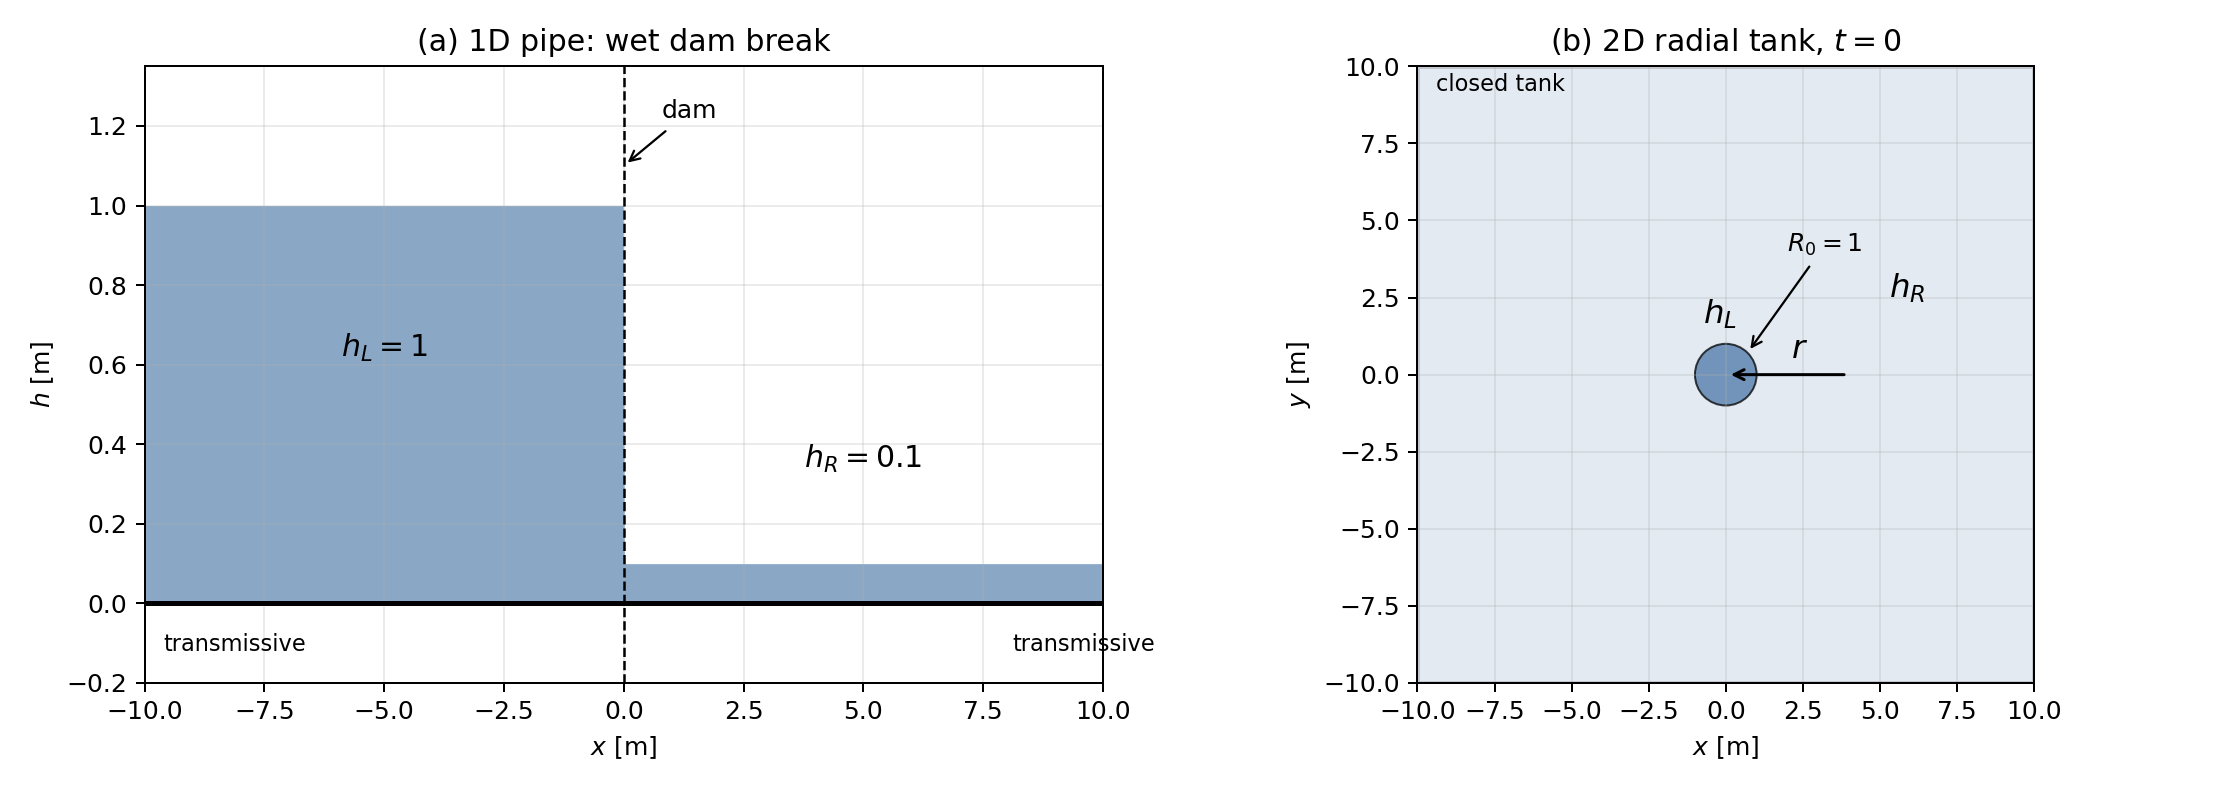
\includegraphics[width=\textwidth]{figures/setup.png}
\caption{Computational setups.  (a) 1D pipe with a wet dam break at $x=0$;
the ends are transmissive.  (b) 2D radial tank with a circular column of
radius $R_0$; the outer boundaries are solid walls.}
\label{fig:setup}
\end{figure}

\begin{table}[H]
\centering
\caption{Computational cases.  All cases use $g=9.81$~m~s$^{-2}$ and a flat
bed.}
\label{tab:cases}
\footnotesize
\setlength{\tabcolsep}{4pt}
\begin{tabular}{@{}l l l l l c c@{}}
\toprule
Case & Domain & Mesh & Initial state & Boundaries & $t_{\rm end}$ [s] & Flux\\
\midrule
\texttt{pipe1D} & $[-10,10]$ & $2000\times1\times1$ & $h_L=1$, $h_R=0.1$ &
transmissive & 1.0 & HLL\\
\texttt{pipe1D\_dry} & $[-10,10]$ & $2000\times1\times1$ & $h_L=1$, $h_R=0$ &
transmissive & 1.0 & HLL\\
\texttt{pipe1D\_nearly} & $[-160,160]$ & $2000\times1\times1$ &
$h_L=1$, $h_R=10^{-3}$ & transmissive & 16.5 & HLL\\
\texttt{radial1D} & $r\in[0,10]$ & $2000\times1\times1$ &
$h_L=1$, $h_R=0.1$, $R_0=1$ & symmetry/transmissive & 2.0 & HLL\\
\texttt{radial2D} & $[-10,10]^2$ & $400\times400\times1$ &
$h_L=1$, $h_R=0.1$, $R_0=1$ & slip walls & 2.0 & HLLC\\
\bottomrule
\end{tabular}
\end{table}

\subsection{Mesh and numerical settings}
The 1D meshes are uniform with $\dx=0.01$~m for the wet and dry pipe,
$\dx=0.16$~m for the long nearly-dry pipe, and $\dr=0.005$~m for the radial
strip.  The 2D mesh is uniform with $\dx=\dy=0.05$~m and one cell in $z$.
The numerical parameters are collected in Table~\ref{tab:params}.  The
\texttt{radial2D} case writes 20 ascii time directories ($\Delta t_{\rm out}=0.1$~s);
the 1D cases write every $0.1$ or $0.5$~s.

\begin{table}[H]
\centering
\caption{Numerical parameters used in the production runs.}
\label{tab:params}
\small
\begin{tabular}{@{}ll@{}}
\toprule
Parameter & Value\\
\midrule
Gravity $g$ & $9.81$~m~s$^{-2}$\\
CFL number & $0.1$\\
Maximum time step & $0.01$~s\\
Depth floor $h_{\min}$ & $10^{-10}$~m\\
Dry tolerance & $10^{-8}$~m\\
First-order fallback depth $h_{\rm recon}$ & $10^{-4}$~m\\
Reconstruction & MUSCL, primitive $(h,u,v)$\\
Limiter & Barth--Jespersen\\
Riemann solver & HLL (1D), HLLC (2D)\\
Time integration & forward Euler\\
\bottomrule
\end{tabular}
\end{table}

\subsection{Boundary and initial conditions}
The initial fields are set with \texttt{setFields}: a box for the 1D cases and
a \texttt{cylinderToCell} for the 2D case.  The 1D pipe uses zero-gradient
\texttt{h} and \texttt{hU}; the radial strip uses symmetry at $r=0$ and
zero-gradient at $r=10$; the 2D tank uses zero-gradient \texttt{h} and slip
\texttt{hU} on all four outer patches.  The initial velocity is zero
everywhere.

\subsection{Verification strategy and metrics}
The verification uses:
\begin{enumerate}[leftmargin=1.4em,itemsep=1pt,topsep=2pt]
\item the Stoker solution \eqref{eq:stoker_h2}--\eqref{eq:stoker_fan} for the
      wet and nearly-dry cases, and the Ritter solution \eqref{eq:ritter} for
      the dry case;
\item the plateau depth $h_2$ (median over the constant region), the plateau
      velocity $u_2$, and the shock position $c_s$ (the crossing of
      $h=\tfrac12(h_2+h_R)$);
\item the $L_1$ error on the cell centres,
      $L_1(q)=\frac{1}{N}\sum_i|q_i-q_{\rm exact}(x_i)|$, and the observed
      order $p=\log(e_N/e_{2N})/\log 2$;
\item the mass $M=\sum_i h_iV_i$ and, for the 2D case, the axial-symmetry
      errors $\max|h(x,y)-h(-x,y)|$, $\max|h(x,y)-h(x,-y)|$, and
      $\max|h(x,y)-h(y,x)|$;
\item the 1D/2D radial comparison at $t=2$~s.
\end{enumerate}
The computations were run in Ubuntu under WSL with OpenFOAM 2406, compiled
with \texttt{g++ -O3}.  The 1D cases take seconds; the $400\times400$ 2D case
takes roughly 10--15 minutes on one core.

%-----------------------------------------------------------------------
\section{Results}
\label{sec:results}

\subsection{Wet, dry, and nearly-dry dam break}
Figure~\ref{fig:allcases} compares the numerical profiles with the exact
solutions.  The wet case (top left) reproduces the rarefaction, the constant
plateau, and the shock; the shock is smeared over a few cells by the HLL
diffusion, but the plateau values are accurate.  The dry case (top right)
follows the Ritter parabola and remains non-negative; the front is smeared
ahead of the exact position.  The nearly-dry case (bottom left) matches the
Stoker solution over the long domain, including the plateau and the shock.
The 1D radial solution (bottom right) is discussed in
Section~\ref{sec:radial1d}.

\begin{figure}[t]
\centering
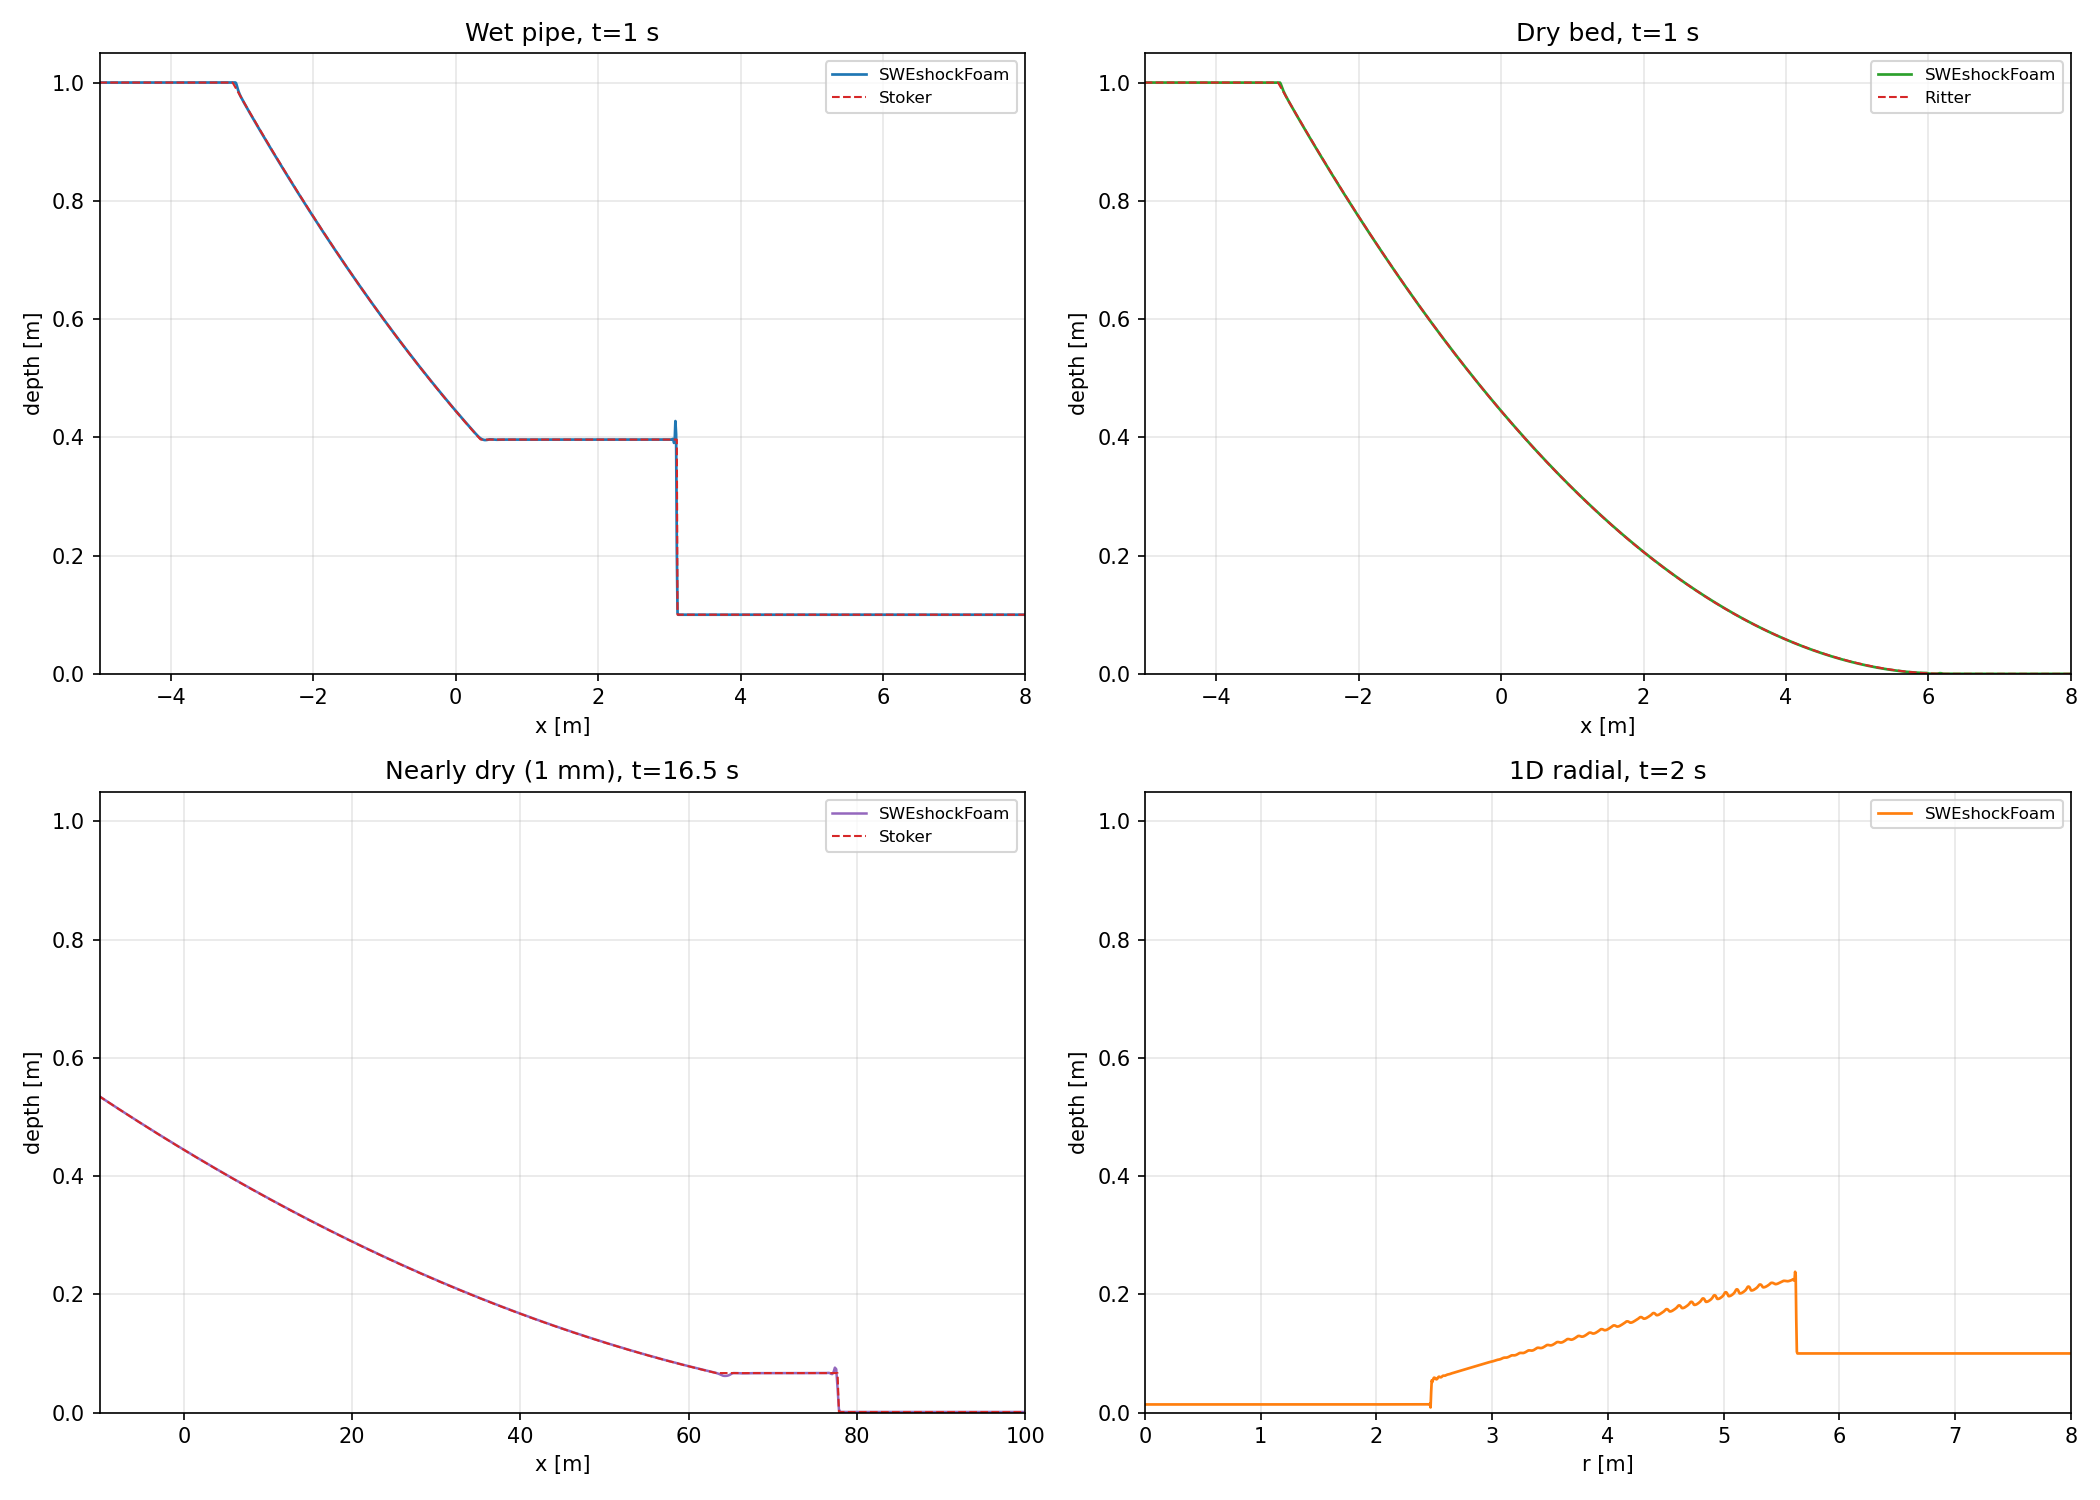
\includegraphics[width=0.92\textwidth]{figures/all_cases.png}
\caption{Verification of the 1D solver.  Top left: wet pipe at $t=1$~s
(Stoker).  Top right: dry bed at $t=1$~s (Ritter).  Bottom left: nearly dry
($h_R=1$~mm) at $t=16.5$~s (Stoker).  Bottom right: 1D axisymmetric radial
dam break at $t=2$~s.  Dashed lines are the exact solutions where available.}
\label{fig:allcases}
\end{figure}

Table~\ref{tab:verification} collects the quantitative comparison.  For the
wet case the relative errors in $h_2$, $u_2$, and $c_s$ are
$+0.001\%$, $+0.005\%$, and $-0.068\%$, respectively.  For the nearly-dry
case the corresponding errors are $-0.090\%$, $+0.061\%$, and $-0.118\%$.
The dry case has no plateau; its front is measured by the $h>10^{-6}$~m
crossing and overestimates the exact front by $5.8\%$ because of the numerical
diffusion.  The depth remains positive ($h_{\min}=10^{-10}$~m), the maximum
depth is $1.000034$~m, and the mass is conserved to round-off.

\begin{table}[H]
\centering
\caption{Verification against the exact Ritter/Stoker solutions.  The error is
relative to the exact value; the dry front uses the $h>10^{-6}$~m crossing and
is therefore a conservative (ahead-of-front) measure.}
\label{tab:verification}
\small
\begin{tabular}{@{}llrrr@{}}
\toprule
Case & Quantity & Exact & Numerical & Error [\%]\\
\midrule
wet, $t=1$ & $h_2$ [m] & 0.396175 & 0.396180 & $+0.001$\\
wet, $t=1$ & $u_2$ [m~s$^{-1}$] & 2.321355 & 2.321479 & $+0.005$\\
wet, $t=1$ & $c_s$ [m~s$^{-1}$] & 3.105134 & 3.103032 & $-0.068$\\
nearly dry, $t=16.5$ & $h_2$ [m] & 0.066830 & 0.066770 & $-0.090$\\
nearly dry, $t=16.5$ & $u_2$ [m~s$^{-1}$] & 4.644801 & 4.647626 & $+0.061$\\
nearly dry, $t=16.5$ & $c_s$ [m~s$^{-1}$] & 4.715359 & 4.709773 & $-0.118$\\
dry, $t=1$ & front [m] & 6.264184 & 6.625000 & $+5.76$\\
\bottomrule
\end{tabular}
\end{table}

The wet and nearly-dry results are essentially exact at the level of the
integrated quantities, which validates the flux, the reconstruction, and the
time step.  The dry case is more demanding: the HLL diffusion smears the
moving front, and the $h>10^{-6}$~m metric is sensitive to the tail.  The
positivity treatment is nevertheless effective: no negative depth appears,
and the mass error is at the level of round-off.

\subsection{Grid convergence}
The wet dam break was recomputed on meshes with
$N=128,256,512,1024,2048$ cells, keeping $\mathrm{CFL}=0.1$ and all other
parameters fixed.  Figure~\ref{fig:convergence} shows the $L_1$ errors of
$h$ and $hu$; Table~\ref{tab:convergence} lists the values and the observed
orders.  The $L_1$ error decreases by roughly a factor of two per mesh
refinement, with observed orders between $0.76$ and $1.18$ for $h$ and
between $0.52$ and $1.50$ for $hu$; the average is about $0.9$.  This is the
expected behaviour for a shock-dominated solution: the MUSCL scheme is
second order in smooth regions by construction, while the shock
contributes a first-order $L_1$ error that dominates the norm.  The $L_\infty$ error is dominated by the
shock position and does not decrease monotonically; it is therefore not a
useful convergence metric here.

\begin{figure}[H]
\centering
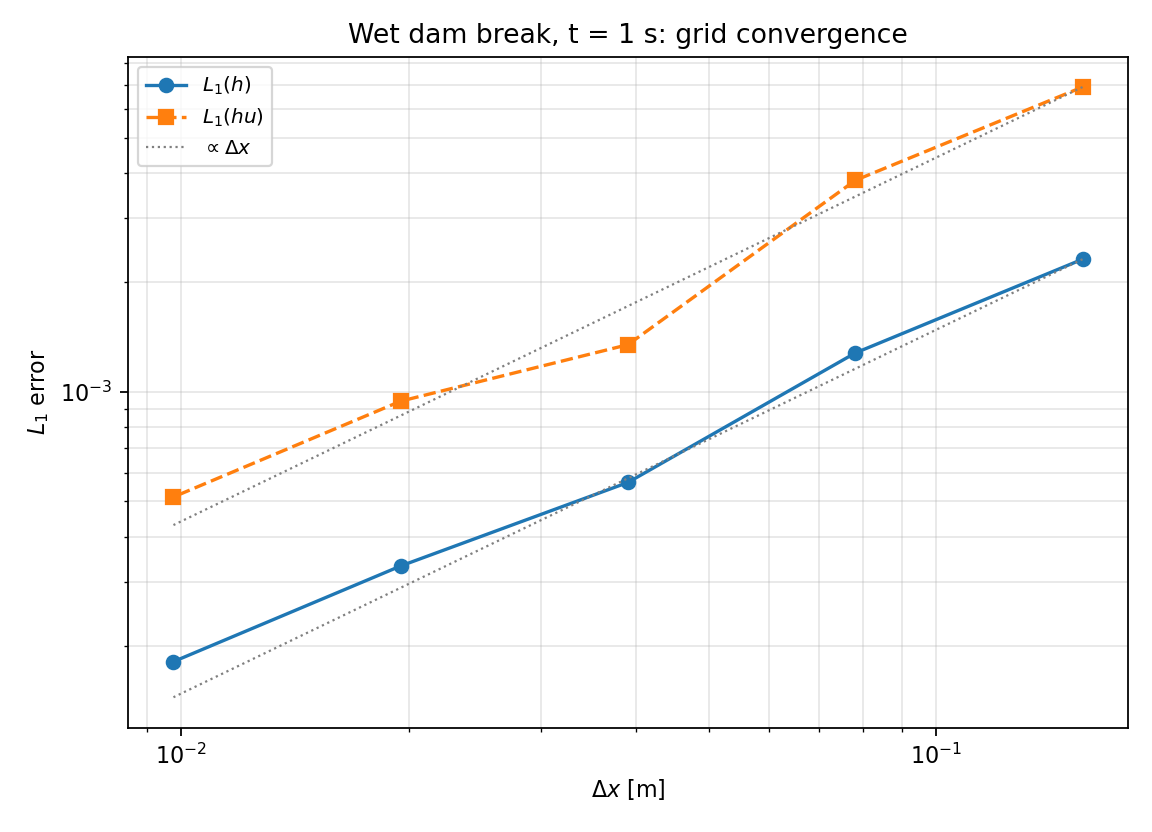
\includegraphics[width=0.72\textwidth]{figures/convergence.png}
\caption{Grid convergence of the wet dam break at $t=1$~s: $L_1$ errors of
$h$ and $hu$ versus the mesh spacing $\dx$.  The dotted line is a reference
$\propto\dx$ slope.}
\label{fig:convergence}
\end{figure}

\begin{table}[H]
\centering
\caption{Grid-convergence data for the wet dam break.  The observed order is
$p=\log(e_N/e_{2N})/\log2$.}
\label{tab:convergence}
\small
\begin{tabular}{@{}rrrrrr@{}}
\toprule
$N$ & $\dx$ [m] & $L_1(h)$ & $p_h$ & $L_1(hu)$ & $p_{hu}$\\
\midrule
128  & 0.15625   & $2.317\times10^{-3}$ & 0.86 & $6.891\times10^{-3}$ & 0.85\\
256  & 0.078125  & $1.280\times10^{-3}$ & 1.18 & $3.817\times10^{-3}$ & 1.50\\
512  & 0.0390625 & $5.641\times10^{-4}$ & 0.76 & $1.349\times10^{-3}$ & 0.52\\
1024 & 0.0195313 & $3.324\times10^{-4}$ & 0.87 & $9.435\times10^{-4}$ & 0.87\\
2048 & 0.0097656 & $1.814\times10^{-4}$ & --   & $5.145\times10^{-4}$ & --\\
\bottomrule
\end{tabular}
\end{table}

\subsection{One-dimensional axisymmetric radial dam break}
\label{sec:radial1d}
Figure~\ref{fig:radialevolution} shows the radial depth and velocity at
$t=0.5$, $1$, and $2$~s.  The initial column produces an outward shock (the
outer circle) and an inward rarefaction that reaches the axis and is reflected
as an inner bore.  By $t=2$~s the inner bore is at $r\approx2.5$~m and the
outer shock is at $r\approx5.6$~m.  The depth rises from about $0.014$~m at
the centre to $0.238$~m at the outer plateau and drops to the ambient
$0.1$~m across the shock.  The radial velocity reaches a maximum of about
$1.39$~m~s$^{-1}$.

\begin{figure}[H]
\centering
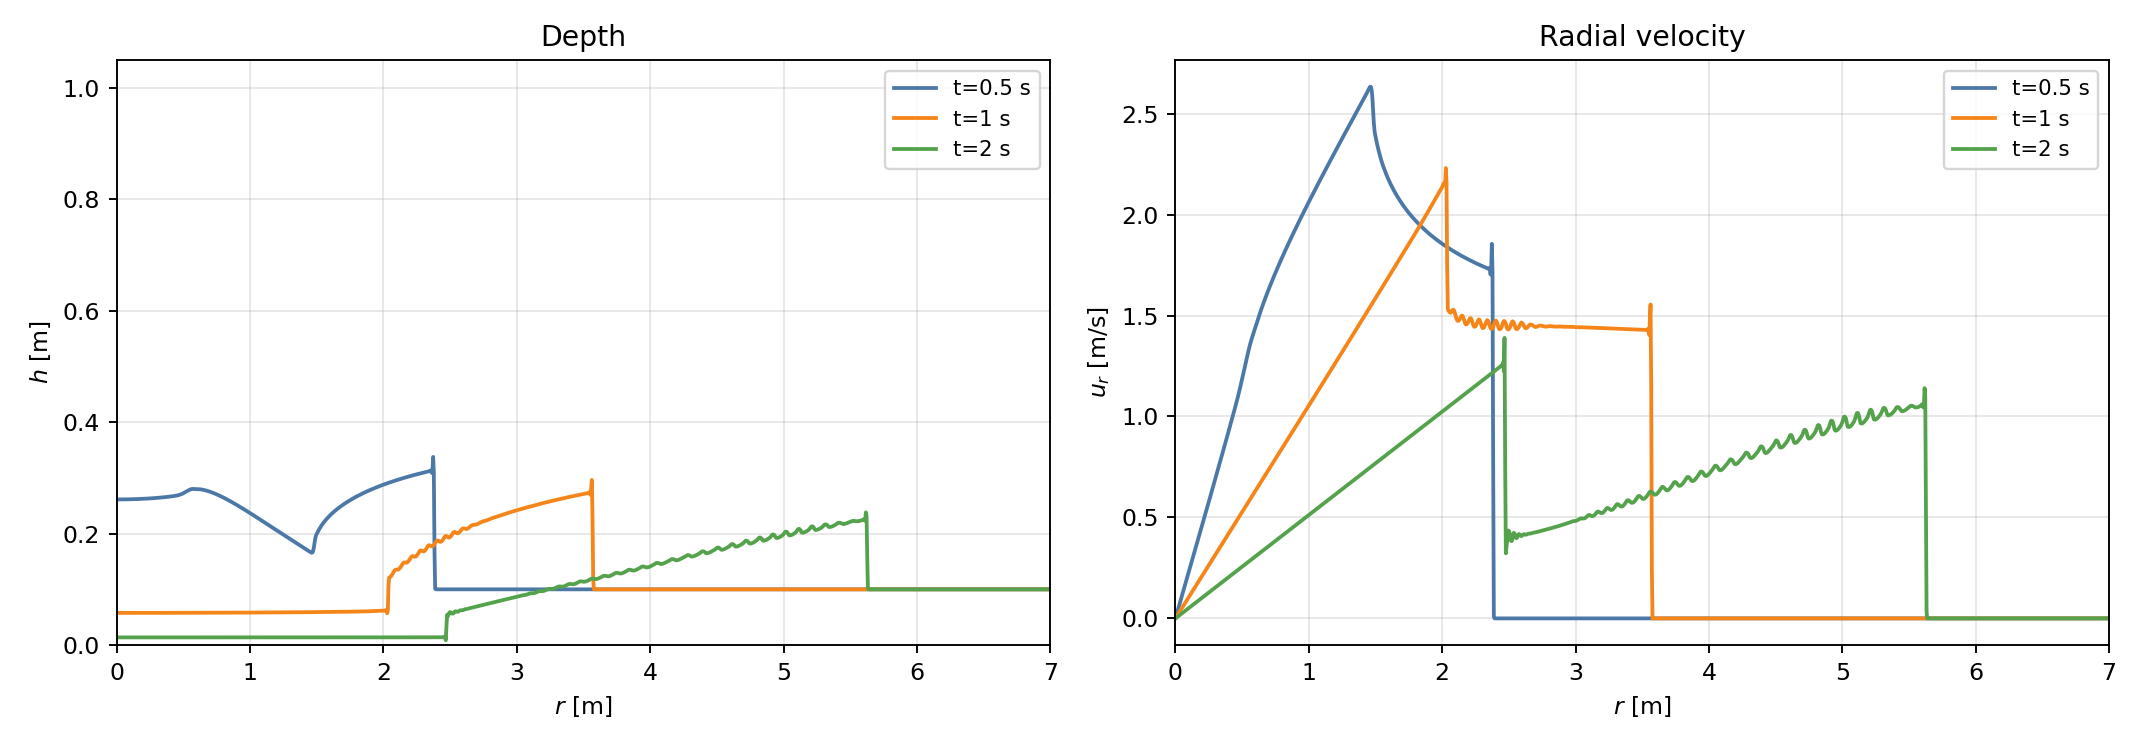
\includegraphics[width=\textwidth]{figures/radial_evolution.png}
\caption{1D axisymmetric radial dam break: depth (left) and radial velocity
(right) at $t=0.5$, $1$, and $2$~s.  The inward rarefaction, the inner bore,
and the outward shock are visible.}
\label{fig:radialevolution}
\end{figure}

The 1D radial run is stable and conserves mass: the discrete mass
$2\pi\sum_i r_i h_i\Delta r$ is constant to round-off, and the lake-at-rest
balance \eqref{eq:lake} is exact.  The main deficiency is a small sawtooth in
$u_r$ on the outer plateau (visible in the right panel of
Figure~\ref{fig:radialevolution}).  The depth profile is smooth; the velocity
oscillation is a residual of the Barth--Jespersen limiter and the cell-centred
geometric source.  The amplitude is about $2\%$ of $u_r$ and does not affect
the front position or the mass.

\subsection{Two-dimensional radial dam break}
Figure~\ref{fig:radialcompare} compares the 2D solution at $t=2$~s with the
1D axisymmetric reference.  The 2D depth map is a circular bore; the radial
average of the 2D field almost coincides with the 1D profile.  The 2D field is
axisymmetric to machine precision: the maximum differences under
$x$-reflection, $y$-reflection, and $x\leftrightarrow y$ transpose are all
zero.  The mass is conserved to $1.2\times10^{-10}$ relative error.

\begin{figure}[t]
\centering
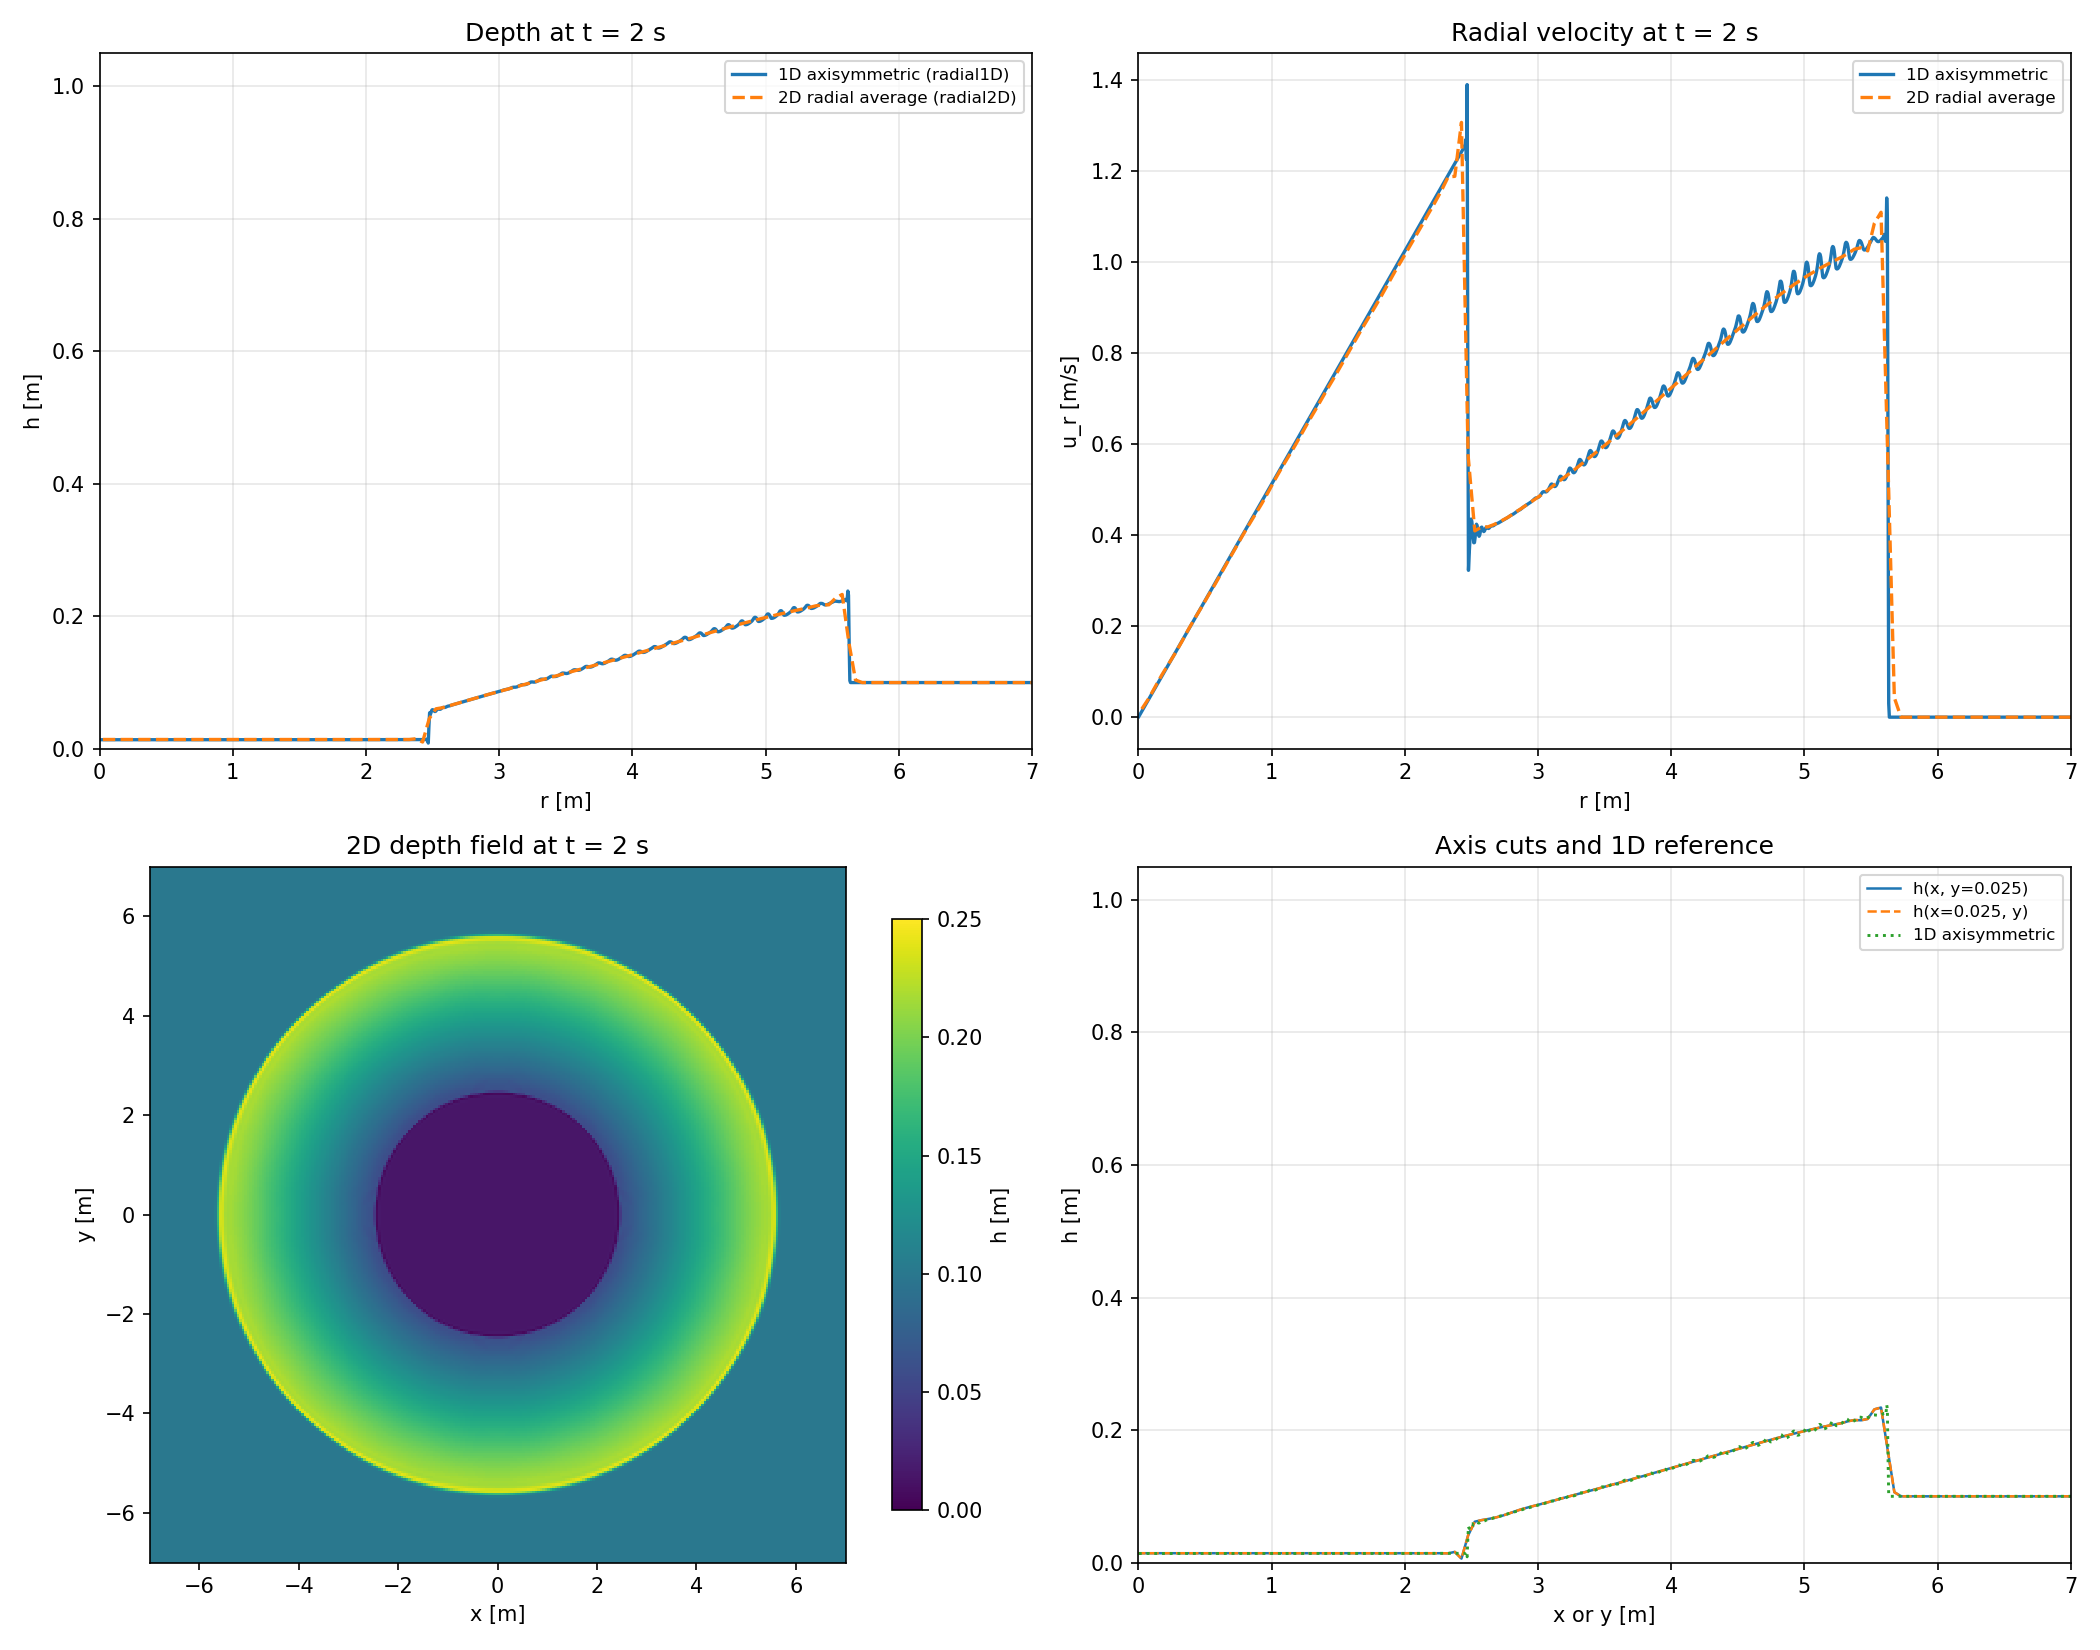
\includegraphics[width=0.92\textwidth]{figures/radial_1d_vs_2d.png}
\caption{1D axisymmetric versus 2D radial dam break at $t=2$~s.  Top:
depth and radial velocity; the dashed line is the radial average of the 2D
field.  Bottom left: 2D depth field on the $400\times400$ mesh.  Bottom right:
axis cuts and the 1D reference.}
\label{fig:radialcompare}
\end{figure}

Table~\ref{tab:radial} lists the quantitative comparison.  The front position
is $5.625$~m in 2D versus $5.6275$~m in 1D (a $0.04\%$ difference); the centre
depth is $0.01411$~m versus $0.01374$~m ($+2.7\%$); the maximum depth is
$0.2330$~m versus $0.2381$~m ($-2.1\%$); the maximum radial velocity is
$1.306$~m~s$^{-1}$ versus $1.389$~m~s$^{-1}$ ($-6.0\%$).  The differences are
consistent with the resolution: the 1D radial mesh has $\dr=5$~mm, while the
2D mesh has $\dx=50$~mm across the initial column, i.e.\ only about 20 cells
across the radius $R_0$.

\begin{table}[H]
\centering
\caption{1D axisymmetric versus 2D radial dam break at $t=2$~s.  The last
column is the relative difference $(q_{2D}/q_{1D}-1)\times100\%$.}
\label{tab:radial}
\small
\begin{tabular}{@{}lrrr@{}}
\toprule
Quantity & 1D & 2D & Difference [\%]\\
\midrule
$h_{\rm centre}$ [m] & 0.013742 & 0.014110 & $+2.68$\\
$h_{\max}$ [m] & 0.238120 & 0.233014 & $-2.14$\\
$r_{\rm front}$ [m] & 5.6275 & 5.6250 & $-0.04$\\
$h_{\rm front}$ [m] & 0.157476 & 0.160661 & $+2.02$\\
$u_{\max}$ [m~s$^{-1}$] & 1.38928 & 1.30635 & $-5.97$\\
$h_{\min}$ [m] & 0.008682 & 0.004379 & --\\
\bottomrule
\end{tabular}
\end{table}

The 2D result is a strong verification of the implementation: an exactly
axisymmetric initial condition on a square Cartesian mesh produces an exactly
axisymmetric field, and the radial profile agrees with the independent 1D
axisymmetric solver.  The remaining differences are resolution effects, not a
loss of symmetry.

\subsection{Limitations of the preliminary results}
The results above are preliminary in several respects.
\begin{enumerate}[leftmargin=1.4em,itemsep=1pt,topsep=2pt]
\item The stable CFL number is $0.1$.  The forward-Euler/MUSCL combination is
      not stable at the more usual $0.4$ on these cases; a second-order
      Runge--Kutta or SSP time integrator would allow a larger time step and is
      left for the final report.
\item The HLL solver is diffusive.  The dry front is smeared by about
      $0.36$~m in the $h>10^{-6}$~m metric, and the $L_1$ convergence is
      first order because of the shock.
\item The radial velocity retains a small sawtooth on the outer plateau; a
      smoother limiter or a fully well-balanced radial source is future work.
\item The 2D mesh is coarse ($400\times400$, $\dx=50$~mm).  A 2D mesh
      refinement study and the Clawpack $2:1$ benchmark are not yet included;
      the 1D/2D comparison is the current verification.
\item The model is inviscid, non-dispersive, and flat-bed.  Bed slopes,
      friction, wetting/drying over arbitrary topography, and non-hydrostatic
      effects are outside the present scope.
\end{enumerate}

%-----------------------------------------------------------------------
\section{Conclusions}
\label{sec:conclusions}

A compact explicit finite-volume shallow-water solver has been implemented in
OpenFOAM and verified on the classical dam-break problems.  The solver uses
HLL/HLLC fluxes, MUSCL reconstruction with a Barth--Jespersen limiter, forward
Euler, a CFL condition, a positivity/dry-bed treatment, and an $r$-weighted
axisymmetric mode.  The wet and nearly-dry cases reproduce the Stoker plateau
and shock to better than $0.1\%$ in the integrated quantities; the dry case
remains positive and mass-conservative, with a diffusive front; and the grid
convergence is consistent with first-order $L_1$ accuracy for a shock-dominated
solution.  The 1D axisymmetric radial solution is stable, and the 2D Cartesian
solution is exactly axisymmetric and agrees with it at the few-percent level.
The main limitations are the small stable CFL number, the diffusive dry front,
the residual radial-velocity sawtooth, and the coarse 2D mesh.

The final report will add: (i) the Clawpack $2:1$ wet radial benchmark after
scaling; (ii) a 2D mesh-refinement study and a quantitative symmetry/mass
convergence table; (iii) a second-order SSP time integrator and a systematic
CFL study; (iv) a smoother/well-balanced radial reconstruction to remove the
sawtooth; and (v) an extension to bed slopes, friction, and wetting/drying for
a more realistic shallow-water application.

%-----------------------------------------------------------------------
\begin{thebibliography}{99}

\bibitem{ritter1892}
A.~Ritter.
\newblock Die Fortpflanzung der Wasserwellen.
\newblock \emph{Zeitschrift des Vereines Deutscher Ingenieure},
  36(33):947--954, 1892.

\bibitem{stoker1957}
J.~J. Stoker.
\newblock \emph{Water Waves: The Mathematical Theory with Applications}.
\newblock Interscience, New York, 1957.

\bibitem{toro2009}
E.~F. Toro.
\newblock \emph{Riemann Solvers and Numerical Methods for Fluid Dynamics}.
\newblock Springer, Berlin, 3rd edition, 2009.

\bibitem{leveque2002}
R.~J. LeVeque.
\newblock \emph{Finite Volume Methods for Hyperbolic Problems}.
\newblock Cambridge University Press, Cambridge, 2002.

\bibitem{harten1983}
A.~Harten, P.~D. Lax, and B.~van Leer.
\newblock On upstream differencing and Godunov-type schemes for hyperbolic
  conservation laws.
\newblock \emph{SIAM Review}, 25(1):35--61, 1983.

\bibitem{toro1994}
E.~F. Toro, M.~Spruce, and W.~Speares.
\newblock Restoration of the contact surface in the HLL-Riemann solver.
\newblock \emph{Shock Waves}, 4(1):25--34, 1994.

\bibitem{vanleer1979}
B.~van Leer.
\newblock Towards the ultimate conservative difference scheme. V. A second-order
  sequel to Godunov's method.
\newblock \emph{Journal of Computational Physics}, 32(1):101--136, 1979.

\bibitem{barth1989}
T.~J. Barth and D.~C. Jespersen.
\newblock The design and application of upwind schemes on unstructured meshes.
\newblock AIAA Paper 89-0366, 1989.

\bibitem{audusse2004}
E.~Audusse, F.~Bouchut, M.-O. Bristeau, R.~Klein, and B.~Perthame.
\newblock A fast and stable well-balanced scheme with hydrostatic reconstruction
  for shallow water flows.
\newblock \emph{SIAM Journal on Scientific Computing}, 25(6):2050--2065, 2004.

\bibitem{kurganov2007}
A.~Kurganov and G.~Petrova.
\newblock A second-order well-balanced positivity preserving central-upwind
  scheme for the Saint-Venant system.
\newblock \emph{Communications in Mathematical Sciences}, 5(1):133--160, 2007.

\bibitem{bollermann2013}
A.~Bollermann, G.~Chen, A.~Kurganov, and S.~Noelle.
\newblock A well-balanced reconstruction of wet/dry fronts for the shallow water
  equations.
\newblock \emph{Journal of Scientific Computing}, 56(2):267--290, 2013.

\bibitem{delestre2013}
O.~Delestre, C.~Lucas, P.-A. Ksinant, F.~Darboux, C.~Laguerre, T.-N.-T. Vo,
  F.~James, and S.~Cordier.
\newblock SWASHES: a compilation of shallow water analytic solutions for
  hydraulic and hydrology.
\newblock \emph{International Journal for Numerical Methods in Fluids},
  72(3):269--300, 2013.

\bibitem{mandli2016}
K.~T. Mandli, A.~J. Ahmadia, M.~Berger, D.~Calhoun, D.~L. George,
  Y.~Hadjimichael, D.~I. Ketcheson, G.~I. Lemoine, and R.~J. LeVeque.
\newblock Clawpack: building an open source ecosystem for solving hyperbolic
  PDEs.
\newblock \emph{PeerJ Computer Science}, 2:e68, 2016.

\bibitem{weller1998}
H.~G. Weller, G.~Tabor, H.~Jasak, and C.~Fureby.
\newblock A tensorial approach to computational continuum mechanics using
  object-oriented techniques.
\newblock \emph{Computers in Physics}, 12(6):620--631, 1998.

\bibitem{openfoam2406}
OpenCFD Ltd.
\newblock OpenFOAM v2406 user and developer documentation.
\newblock \url{https://www.openfoam.com}, 2026.
\newblock Accessed November 2026.

\end{thebibliography}

%-----------------------------------------------------------------------
\clearpage
\appendix
\section{Program listing}

The full solver is part of the project repository.  Its source is
\begin{center}
\texttt{solvers/SWEshockFoam/SWEshockFoam.C}
\end{center}
The code is available at
\url{https://github.com/Illus1onist/SWEshockCatcher}.
The two excerpts below
show the HLLC flux and the conservative face-to-cell update, which are the
core of the method.  The complete application is compiled with
\texttt{wmake} and run with the case \texttt{Allrun} scripts.

\lstinputlisting[language=C++, firstline=84, lastline=141, firstnumber=84,
  caption={HLLC Riemann flux (three waves, tangential velocity carried through
  the contact).}, label={lst:hllc}]
  {../solvers/SWEshockFoam/SWEshockFoam.C}

\clearpage
\lstinputlisting[language=C++, firstline=393, lastline=431, firstnumber=393,
  caption={Conservative update: owner/neighbour flux orientation, radial
  source, positivity floor, and dry treatment.}, label={lst:update}]
  {../solvers/SWEshockFoam/SWEshockFoam.C}

\section{Reproducibility}

The main commands are
\begin{verbatim}
cd solvers/SWEshockFoam && wmake
cd SWEshockFoam/pipe1D && ./Allrun
cd SWEshockFoam/radial1D && ./Allrun
cd SWEshockFoam/radial2D && ./Allrun
\end{verbatim}
The 1D grid-convergence data are reproduced with
\begin{verbatim}
cd SWEshockFoam/convergence && ./run_convergence.sh
python3 analyze_convergence.py
\end{verbatim}
The analysis scripts read the OpenFOAM ascii fields and require
\texttt{numpy} and \texttt{matplotlib}.

\end{document}

